\documentclass[a4paper,twocolumn]{article}
\usepackage[hmargin={1.1cm,1.1cm},vmargin={2.2cm,2cm}]{geometry}
%       includehead,     scale=0.85,centering,hoffset=-0.1cm,voffset=-0.5cm]{geometry} headheight=13.1pt ,portrait

%\usepackage[a4paper,portrait,twocolumn,includeheadfoot,
%            scale=0.85,centering,hoffset=-1cm]{geometry}
\usepackage[pdftex]{graphicx,color}
\usepackage{amsmath}
\usepackage{amssymb}
\usepackage{stmaryrd}
\usepackage[french]{babel}
\selectlanguage{french}
\usepackage{fancyhdr}
\usepackage{floatflt}
\usepackage{ucs}
\usepackage[utf8]{inputenc}
\usepackage[T1]{fontenc}
\usepackage[pdftex,colorlinks={true},urlcolor={blue},pdfauthor={remy Nicolai}]{hyperref}
\usepackage{makeidx}


%Options de hyperref pour les fichiers pdf g{\'e}n{\'e}r{\'e}s
%\hypersetup{pdfpagemode=None,colorlinks=true,pdffitwindow=true}
%\hypersetup{pdfpagemode=None,colorlinks=true}


%                 Chargement des symboles de l'AMS
%\input amssym
%pour que la compilation aille au bout
%\nofiles\scrollmode

%pr{\'e}sentation du compteur de niveau 2 dans les listes
\makeatletter
\renewcommand{\labelenumii}{\theenumii.}
\makeatother

%dimension des pages, en-t{\^e}te et bas de page
  %utilisation avec vmargin
   %\setpapersize{custom}{21cm}{29.7cm}
   %\setmarginsrb{1.5cm}{0cm}{3.5cm}{1cm}{15mm}{10mm}{0mm}{0mm}
%\setlength{\voffset}{-2cm}
%\setlength{\oddsidemargin}{-1cm}
%\setlength{\textheight}{25cm}
%\setlength{\textwidth}{17.3cm}
%\columnsep=5pt
% \columnseprule=0.5pt
%\columnseprule=0.5pt
%En tete et pied de page
\pagestyle{fancy}
\lhead{Lycée Hoche MPSI B}
%\rhead{}
%\rhead{25/11/05}
\lfoot{\tiny{Cette création est mise à disposition selon le Contrat\\ Paternité-Partage des Conditions Initiales à l'Identique 2.0 France\\ disponible en ligne http://creativecommons.org/licenses/by-sa/2.0/fr/
} }
\rfoot{\tiny{Rémy Nicolai \jobname pdf du \today}}

%\pagestyle{fancy}
%\lhead{MPSI B}
%\rhead{\today}
%\rfoot{\small{\jobname}}
\newcommand{\baseurl}{http://back.maquisdoc.net/data/}
\newcommand{\textesurl}{http://back.maquisdoc.net/data/devoirs_nicolair/}
\newcommand{\exosurl}{http://back.maquisdoc.net/data/exos_nicolair/}
\newcommand{\coursurl}{http://back.maquisdoc.net/data/cours_nicolair/}

\newcommand{\N}{\mathbb{N}}
\newcommand{\Z}{\mathbb{Z}}
\newcommand{\C}{\mathbb{C}}
\newcommand{\R}{\mathbb{R}}
\newcommand{\K}{\mathbf{K}}
\newcommand{\Q}{\mathbb{Q}}
\newcommand{\F}{\mathbf{F}}
\newcommand{\U}{\mathbb{U}}
\newcommand{\p}{\mathbb{P}}


\newcommand{\card}{\mathop{\mathrm{Card}}}
\newcommand{\Id}{\mathop{\mathrm{Id}}}
\newcommand{\Ker}{\mathop{\mathrm{Ker}}}
\newcommand{\Vect}{\mathop{\mathrm{Vect}}}
\newcommand{\cotg}{\mathop{\mathrm{cotan}}}
\newcommand{\cotan}{\mathop{\mathrm{cotan}}}
\newcommand{\sh}{\mathop{\mathrm{sh}}}
\newcommand{\ch}{\mathop{\mathrm{ch}}}
\newcommand{\argch}{\mathop{\mathrm{argch}}}
\newcommand{\argsh}{\mathop{\mathrm{argsh}}}
\newcommand{\tr}{\mathop{\mathrm{tr}}}
\newcommand{\rg}{\mathop{\mathrm{rg}}}
\newcommand{\rang}{\mathop{\mathrm{rg}}}
\newcommand{\val}{\mathop{\mathrm{val}}}

\newcommand{\Mat}{\mathop{\mathrm{Mat}}}
\newcommand{\MatB}[2]{\mathop{\mathrm{Mat}}_{\mathcal{#1}}\left( #2\right) }
\newcommand{\MatBB}[3]{\mathop{\mathrm{Mat}}_{\mathcal{#1} \mathcal{#2}}\left( #3\right) }

\renewcommand{\Re}{\mathop{\mathrm{Re}}}
\newcommand{\Ima}{\mathop{\mathrm{Im}}}
\renewcommand{\Im}{\mathop{\mathrm{Im}}}
\renewcommand{\th}{\mathop{\mathrm{th}}}
\newcommand{\repere}{$(O,\overrightarrow{i},\overrightarrow{j},\overrightarrow{k})$ }
\newcommand{\trans}{\mathstrut^t\!}
\newcommand{\cov}{\mathop{\mathrm{Cov}}}
\newcommand{\orth}[1]{#1^{\perp}}

\newcommand{\absolue}[1]{\left| #1 \right|}
\newcommand{\fonc}[5]{#1 : \begin{cases}#2 &\rightarrow #3 \\ #4 &\mapsto #5 \end{cases}}
\newcommand{\depar}[2]{\dfrac{\partial #1}{\partial #2}}
\newcommand{\norme}[1]{\left\| #1 \right\|}
\newcommand{\se}{\geq}
\newcommand{\ie}{\leq}
\newcommand{\serie}[1]{\left( \sum {#1}_n \right)_{n\in\N}}

\batchmode
 
\begin{document} 
\chead{ coniques: énoncés.}
\begin{enumerate}
  \item \begin{tiny}(Eco01)\end{tiny} On considère une parabole $\mathcal P$ d'équation $y^2=px$ avec $p>0$ dans un repère orthonormé. Trouver la longueur minimale d'une corde de $\mathcal P$ normale en une de ses extrémités.

  \item \begin{tiny}(Eco02)\end{tiny} Soient $a$, $b$, $c$, $d$ des réels tels que
\begin{displaymath}
 D = ad - bc \neq 0
\end{displaymath}
 Un repère orthonormé étant fixé; pour tout réel $t$, on note $f(t)$ le point de coordonnées
\begin{displaymath}
 (a\cos t + b\sin t , c\cos t + d\sin t)
\end{displaymath}
Former une équation cartésienne du support de $f$. En déduire qu'il s'agit d'une ellipse. Quel est le support de la courbe lorsque $D=0$?\newline
Pour le point de coordonnées
\begin{displaymath}
 (a\ch t + b\sh t , c\ch t + d\sh t)
\end{displaymath}
quel type de conique obtient-on ?

  \item \begin{figure}[ht]
 \centering
 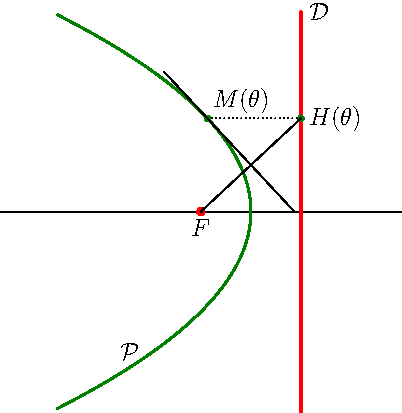
\includegraphics[width=5cm]{Eco03_1.pdf}
 % Eco03_1.pdf: 142x4 px, 72dpi, 5.01x0.14 cm, bb=0 0 142 4
 \caption{Exercice \arabic{enumi} : tangente à une parabole}
 \label{fig:Eco3_1}
\end{figure}

\begin{tiny}(Eco03)\end{tiny} Propriétés des tangentes : parabole.\newline
Dans un plan muni d'un repère orthonormé, on se donne un réel $p>0$, un point $F$ et une parabole $\mathcal P$ paramétrée par :
\begin{displaymath}
 M(\theta) = F + \frac{p}{1+ \cos\theta}\overrightarrow{e_\theta}.
\end{displaymath}
Déterminer des expressions simples de $\lambda(\theta)$ et $\varphi(\theta)$ pour que
\begin{displaymath}
 \overrightarrow{M'}(\theta) = \lambda(\theta)\overrightarrow{e_{\varphi(\theta)}}.
\end{displaymath}
En déduire que la tangente (figure \ref{fig:Eco3_1}) est la médiatrice de $FH(\theta)$. Comment se réfléchit sur $\mathcal P$ un rayon parallèle à l'axe focal ?

  \item \begin{tiny}(Eco04)\end{tiny} Propriétés des tangentes : foyer directrice.\newline
On se donne un point $F$, un vecteur unitaire $\overrightarrow u$ et un réel $\delta$. Soit $f$ une courbe paramétrée $\mathcal{C}^1(I)$.
\begin{enumerate}
 \item Calculer la dérivée en $t\in I$ de la fonction
\begin{displaymath}
 t \rightarrow \frac{\Vert \overrightarrow{Ff(t)}\Vert}{(\overrightarrow{Ff(t)}/\overrightarrow u) - \delta}
\end{displaymath}
\item On suppose que $f$ est une paramétrisation d'une conique d'excentricité $e$, de foyer $F$, d'axe focal $F+\Vect(\overrightarrow u)$ la directrice passe par le point $F+\delta\,\overrightarrow u$. On note :
\begin{itemize}
 \item écart angulaire entre $\overrightarrow u$ et $\overrightarrow{f'(t)}$ : $\varphi$
 \item écart angulaire entre $\overrightarrow{Ff(t)}$ et $\overrightarrow{f'(t)}$ : $\psi$
\end{itemize}
Montrer que 
\begin{displaymath}
 |\cos \psi | = e |\cos \varphi|
\end{displaymath}
Former des relations sans valeur absolue pour les divers cas possibles. Que retrouve-t-on dans le cas de la parabole.
\end{enumerate}

  \item \begin{tiny}(Eco05)\end{tiny} Propriétés des tangentes : définition bifocale.\newline
Soit $F$ et $F'$ deux points distincts et $t\rightarrow f(t)$ une courbe paramétrée $\mathcal{C}^1$ dont le support est une conique $\mathcal C$ de foyers $F$ et $F'$. En calculant les dérivées de
\begin{align*}
 t\rightarrow \Vert \overrightarrow{Ff(t)}\Vert & &
 t\rightarrow \Vert \overrightarrow{F'f(t)}
\end{align*}
montrer que la tangente en $f(t)$ à $\mathcal C$ est une bissectrice (à préciser selon les cas) des droites $(Ff(t))$, $(F'f(t))$.

  \item \begin{figure}[ht]
 \centering
 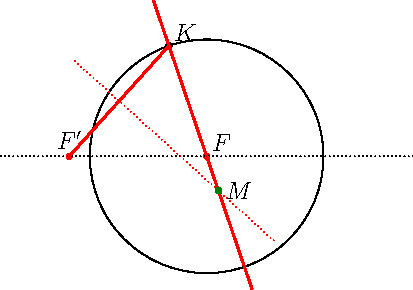
\includegraphics[width=5cm]{Eco06_1.pdf}
 % Eco06_1.pdf: 198x139 px, 72dpi, 6.99x4.90 cm, bb=0 0 198 139
 \caption{Exercice \arabic{enumi} : cas $a<c$}
 \label{fig:Eco6_1}
\end{figure}
\begin{figure}[ht]
 \centering
 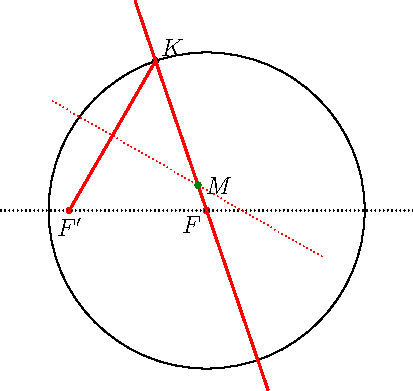
\includegraphics[width=5cm]{Eco06_2.pdf}
 % Eco06_1.pdf: 198x139 px, 72dpi, 6.99x4.90 cm, bb=0 0 198 139
 \caption{Exercice \arabic{enumi} : cas $a>c$}
 \label{fig:Eco6_2}
\end{figure}

\begin{tiny}(Eco06)\end{tiny} Cercle directeur.\newline
Soit $c>0$ et deux points $F$ et $F'$ avec $FF'=2c$, le cercle $\mathcal C$ est centré en $F$ et de rayon $2a$ ($a>0$).\newline
\`A tout point $K$ de $\mathcal C$, on associe le point d'intersection $M$ (lorsqu'il existe) de la médiatrice de $[F',K]$ avec la droite $(KF)$. On devra considérer les deux cas (figure \ref{fig:Eco6_1} et figure \ref{fig:Eco6_2}).
\begin{enumerate}
 \item Préciser le cas dans lequel la médiatrice de $[F',K]$ et la droite $(KF)$ ne se coupent pas.
 \item Montrer que lorsque $K$ décrit $\mathcal C$, le point $M$ décrit une conique à préciser. On dit que $\mathcal C$ est le \emph{cercle directeur} de la conique.
 \item On paramètre le cercle directeur par 
\begin{displaymath}
 \theta \rightarrow K(\theta) = F +2a\overrightarrow{e_\theta}
\end{displaymath}
et on note $M(\theta)$ le point correspondant. Calculer $M(\theta)$ et $\overrightarrow {M'} (\theta)$. En déduire que la médiatrice de $[F'K]$ est la tangente en $M$ à la conique.
\item Quelle est la courbe formée par les projetés orthogonaux de $F'$ sur les tangentes à la conique (podaire) ? \index{podaire}
\end{enumerate}

  \item \begin{tiny}(Eco07)\end{tiny} Une droite coupe une conique en deux points $M_1$ et $M_3$ et sa directrice en $P$. En utilisant la représentation polaire
\begin{displaymath}
 M(\theta) = F + \frac{p}{1+e\cos \theta}\overrightarrow{e}_\theta
\end{displaymath}
 montrer que la droite $(FP)$ est une bissectrice des droites $(FM_1)$ et $(FM_2)$.

  \item \begin{tiny}(Eco08)\end{tiny} Soit $\mathcal C_\theta$ la conique d'équation
\begin{displaymath}
 x^2 \sin^2\theta -xy\sin2\theta + y^2(1+\cos^2\theta) = a^2\sin^2\theta
\end{displaymath}
 où $x$ et $y$ désignent les fonctions coordonnées dans un repère orthonormé et $\theta\not \equiv 0 \mod \pi$.
\begin{enumerate}
 \item Quel est le genre de $\mathcal C$?
 \item On considère un nouveau repère dans lequel les fonctions coordonnées $X$ et $Y$ vérifient
\begin{displaymath}
 \left\lbrace 
\begin{aligned}
 x &= \cos \varphi X +\sin \varphi Y \\
 y &= -\sin \varphi X +\cos \varphi X 
\end{aligned}
\right. 
\end{displaymath}
Déterminer les $\varphi$ pour lesquels le coefficient de $XY$ dans l'équation de $\mathcal C_\theta$ exprimée à l'aide de $X$ et $Y$ est nul.
\item On suppose ici $0<\theta<\frac{\pi}{2}$. Exprimer l'équation de $\mathcal C_\theta$ avec les $X$ et $Y$ obtenus pour $\varphi=-\frac{\theta}{2}$. Montrer qu'il s'agit d'une équation réduite et calculer les foyers de la conique.
\end{enumerate}

  \item \begin{tiny}(Eco09)\end{tiny} Soit $\mathcal{H}$ une hyperbole d'équation réduite
\begin{displaymath}
 \frac{x^2}{a^2} - \frac{y^2}{b^2}=1
\end{displaymath}
 Calculer la distance d'un foyer à une asymptote.

\ \item \begin{tiny}(Eco10)\end{tiny} On considère une hyperbole d'équation réduite
\begin{displaymath}
 \frac{x^2}{a^2}-\frac{y^2}{b^2}=1
\end{displaymath}
où $x$ et $y$ désignent les fonctions coordonnées dans un repère $(O,(\overrightarrow i, \overrightarrow j))$. \'Ecrire les équations des asymptotes à l'aide des fonctions coordonnées relatives aux repères $(F,(\overrightarrow i, \overrightarrow j))$ et $(F',(\overrightarrow i, \overrightarrow j))$ où $F$ et $F'$ sont les deux foyers.
  \item \begin{tiny}(Eco11)\end{tiny} Pour une hyperbole support de la courbe paramétrée
\begin{displaymath}
 f(\theta) = F+\frac{p}{1+e\cos \theta} \overrightarrow e_\theta
\end{displaymath}
 Exprimer les distances centre-sommet $a$, centre-foyer $c$ et le $b$ de l'équation réduite en fonction de $p$ et $e$. 
  \item \begin{tiny}(Eco12)\end{tiny} Courbe orthoptique pour coniques à centre. Cercle de Monge.\\
On considère une conique $\mathcal C$ d'équation réduite
\begin{displaymath}
 \frac{x^2}{a^2}+\varepsilon \,\frac{y^2}{b^2} = 1
\end{displaymath}
 avec $\varepsilon\in \{-1,+1\}$ de manière à couvrir les cas ellipse et hyperbole.\\
Soit $M_0$, de coordonnées $(x_0,y_0)$ un point quelconque du plan et $\overrightarrow u$ de coordonnées $(u,v)$ un vecteur quelconque.
\begin{enumerate}
 \item En admettant qu'une droite est tangente à la conique si et seulement si elle la coupe en deux points confondus, former une condition caractérisant que la droite $M_0+\Vect(\overrightarrow u)$ est tangente à $\mathcal C$.\\
On écrira cette condition sous la former
\begin{displaymath}
Au^2 + Buv + Cv^2 =0
\end{displaymath}
où $A$, $B$, $C$ sont des expressions de $x_0$, $y_0$, $a$, $b$, $\varepsilon$ à déterminer.
\item Lorsque par $M_0$ passent deux tangentes, on note $p_1$ et $p_2$ les pentes de ces droites. Exprimer le produit $p_1p_2$ en fonction de $A$, $B$,$C$ puis de $x_0$, $y_0$, $a$, $b$, $\varepsilon$.
\item Déterminer l'équation de l'ensemble des points $M_0$ par lesquels passent deux tangentes orthogonales. Discuter de l'existence et de la nature de cet ensemble suivant la nature et les caractéristiques de la conique.
\end{enumerate}
  
\end{enumerate}
\clearpage 
\chead{coniques: corrigés.}
\begin{enumerate}
  \item Cco01.tex manque.
  \item Cco02.tex manque.
  \item Calculons la dérivée en introduisant $\frac{\theta}{2}$:
\begin{multline*}
 \overrightarrow{M'}(\theta) = \frac{p\sin \theta}{(1 + \cos \theta)^2} \overrightarrow{e_\theta}
 + \frac{p}{(1 + \cos \theta)} \overrightarrow{e_{\theta + \frac{\pi}{2}}} \\
 = \frac{p}{(1 + \cos \theta)^2} \left( \sin \theta \overrightarrow{e_\theta} + (1+\cos \theta) \overrightarrow{e_{\theta + \frac{\pi}{2}}} \right)\\
 = \frac{2 p \cos \frac{\theta}{2}}{(1 + \cos \theta)^2} \left( \sin \frac{\theta}{2} \overrightarrow{e_\theta} + \cos \frac{\theta}{2} \overrightarrow{e_{\theta + \frac{\pi}{2}}} \right)\\
 = \frac{2 p \cos \frac{\theta}{2}}{(1 + \cos \theta)^2} \left( \cos \frac{\pi - \theta}{2} \overrightarrow{e_\theta} + \sin \frac{\pi - \theta}{2} \overrightarrow{e_{\theta + \frac{\pi}{2}}} \right)\\
 = \frac{2 p \cos \frac{\theta}{2}}{(1 + \cos \theta)^2} \overrightarrow{e_{\frac{\pi + \theta}{2}}}.
\end{multline*}
On en déduit
\begin{displaymath}
 \lambda(\theta) = \frac{2 p \cos \frac{\theta}{2}}{(1 + \cos \theta)^2}, \;\;
 \varphi(\theta) = \frac{\pi + \theta}{2}.
\end{displaymath}


  \item Cco04.tex manque.
  \item Cco05.tex manque.
  \item Cco06.tex manque.
  \item Cco07.tex manque.
  \item Cco08.tex manque.
  \item Par symétries les distances entre les foyers et les asymptotes sont égales pour les deux foyers et asymptotes. Prenons l'asymptote d'équation
\begin{displaymath}
 \frac{x}{a}-\frac{y}{b}=1
\end{displaymath}
et le foyer de coordonnées $(c,0)$. La distance cherchée est
\begin{displaymath}
 \frac{\vert\frac{c}{a} \vert}{\sqrt{\frac{1}{a^2}+\frac{1}{b^2}}}
=\frac{cab}{a\sqrt{a^2+b^2}}=b
\end{displaymath}
car $c^2=a^2+b^2$.

  \item \begin{tiny}(Eco10)\end{tiny} Comme $e=\frac{c}{a}$ et que $X=x\pm c$, on trouve
\begin{displaymath}
 \frac{X}{a}\pm \frac{Y}{b}\pm e =1
\end{displaymath}
Il y a quatre possibilités car deux assymptotes et deux foyers.
  \item Les sommets sont obtenus pour les valeurs $0$ et $\pi$ du paramètre. Ils ont pour abscisse (origine à un foyer)
\begin{displaymath}
 \frac{p}{1+e}\hspace{0.5cm} \frac{p}{e-1}
\end{displaymath}
Le centre est au milieu des deux. On en déduit
\begin{displaymath}
 c=\frac{p}{2}\left(\frac{1}{e+1}+\frac{1}{e-1} \right) = \frac{pe}{e^2-1}
\end{displaymath}
Pour une hyperbole, le sommet $S$ le plus proche de $F$ est entre $F$ et le centre $C$. On en déduit $FS + a =c$. On a $FS=\frac{p}{1+e}$ pour le sommet $S$ le plus proche de $F$. On en déduit
\begin{multline*}
 a=c-FS=\frac{p}{2}\left(-\frac{1}{e+1}+\frac{1}{e-1} \right) = \frac{p}{e^2-1}\\
\Rightarrow
b=\sqrt{c^2-a^2}=\frac{p}{\sqrt{e^2-1}}
\end{multline*}
 
  \item Cco12.tex manque. 
\end{enumerate} 
\end{document}
